\documentclass[twocolumn]{article}
\usepackage[landscape,margin=1cm]{geometry}
\usepackage{hyperref}
\usepackage{graphicx}
\usepackage{amssymb}
\usepackage{amsmath}
\usepackage{natbib}
\bibliographystyle{humannat}
\pagenumbering{gobble}

\begin{document}
\title{\vspace{-1cm}A Galaxy Theorist's T-$\rho$ Phase Guide}
\author{B.\,W. Keller$^1$\thanks{Email: benjamin.keller `at'
uni-heidelberg.de}
\vspace*{6pt}\\
$^1$Zentrum f{\"u}r Astronomie der Universit\"at Heidelberg, Astronomisches
Rechen-Institut,  \\ M{\"o}nchofstra{\ss}e 12-14, D-69120 Heidelberg, Germany\\
}
\maketitle
The this ``cheat-sheet plot'' shows a helpful guide to the eye for the
temperature-density phase diagram of gas in cosmological and galactic
environments.  Temperature and density are shown in units of Kelvin and $m_H
cm^{-3}$, and a number of isocontours are displayed on top of a hexbin histogram
showing the gas within the virial radius of a cosmological simulation of a Milky
Way like galaxy.  This guide is designed to be helpful to theorists and
observers, but betrays a bit of my numerical bias.

The axes are twinned with the sound speed (equation~\ref{sound_speed}) and the
free-fall time (equation~\ref{ff_time}).  Isocontours show a number of useful
values for constant entropy (equation~\ref{entropy}, shown with a black dotted
curve), Jeans mass (equation~\ref{jeans_mass}, shown with a magenta solid
curve), Jeans length (equation~\ref{jeans_length}, shown with a solid gren
curve), Courant time (equation~\ref{courant_time}, shown in a cyan dash-dotted
line), and pressure (equation~\ref{pressure}, shown in a grey dashed line).
Also shown are lines of constant cooling time (in solid blue), and a handful of
interesting densities (in dotted salmon).  All curves assume a solar
metallicity, and a mean molecular weight of $\mu=1$.

The hexbin histogram is taken from g1536, one of the MUGS2 galaxies presented
in \citet{Keller2015,Keller2016}.  The lines of constant cooling time are
derived from the cooling rates first presented in \citet{Shen2010}, now included
as a standard feature in the {\sc Gasoline2} code \citep{Wadsley2017}.

The data and code used to generate this figure, as well as the \LaTeX source for
this document, can be found at \url{https://github.com/bwkeller/phase_guide}. 
\vspace{5cm}
\begin{equation}
c_s = \sqrt{\frac{\gamma k_B T}{\mu m_H}}
\label{sound_speed}
\end{equation}
\begin{equation}
t_{ff} = \left(\frac{3\pi}{32G\mu m_H n}\right)^{1/2}
\label{ff_time}
\end{equation}
\begin{equation}
K = k_BTn^{-2/3}
\label{entropy}
\end{equation}
\begin{equation}
M_J = \left(\mu m_H\right)^{-2}\left(\frac{15k_B}{4\pi G}\right)^{3/2}\left(\frac{T^3}{n}\right)^{1/2}
\label{jeans_mass}
\end{equation}
\begin{equation}
\lambda_J = \left(\mu m_H\right)^{-1}\left(\frac{15k_B}{4\pi G}\right)^{1/2}\left(\frac{T}{n}\right)^{1/2}
\label{jeans_length}
\end{equation}
\begin{equation}
t_{courant} \propto \frac{n^{-1/3}}{c_s}
\label{courant_time}
\end{equation}
\begin{equation}
P = k_B n T
\label{pressure}
\end{equation}
\bibliography{references}
\begin{figure}[hbtp]
\centering
\vspace*{-1cm}
\hspace*{-1cm}
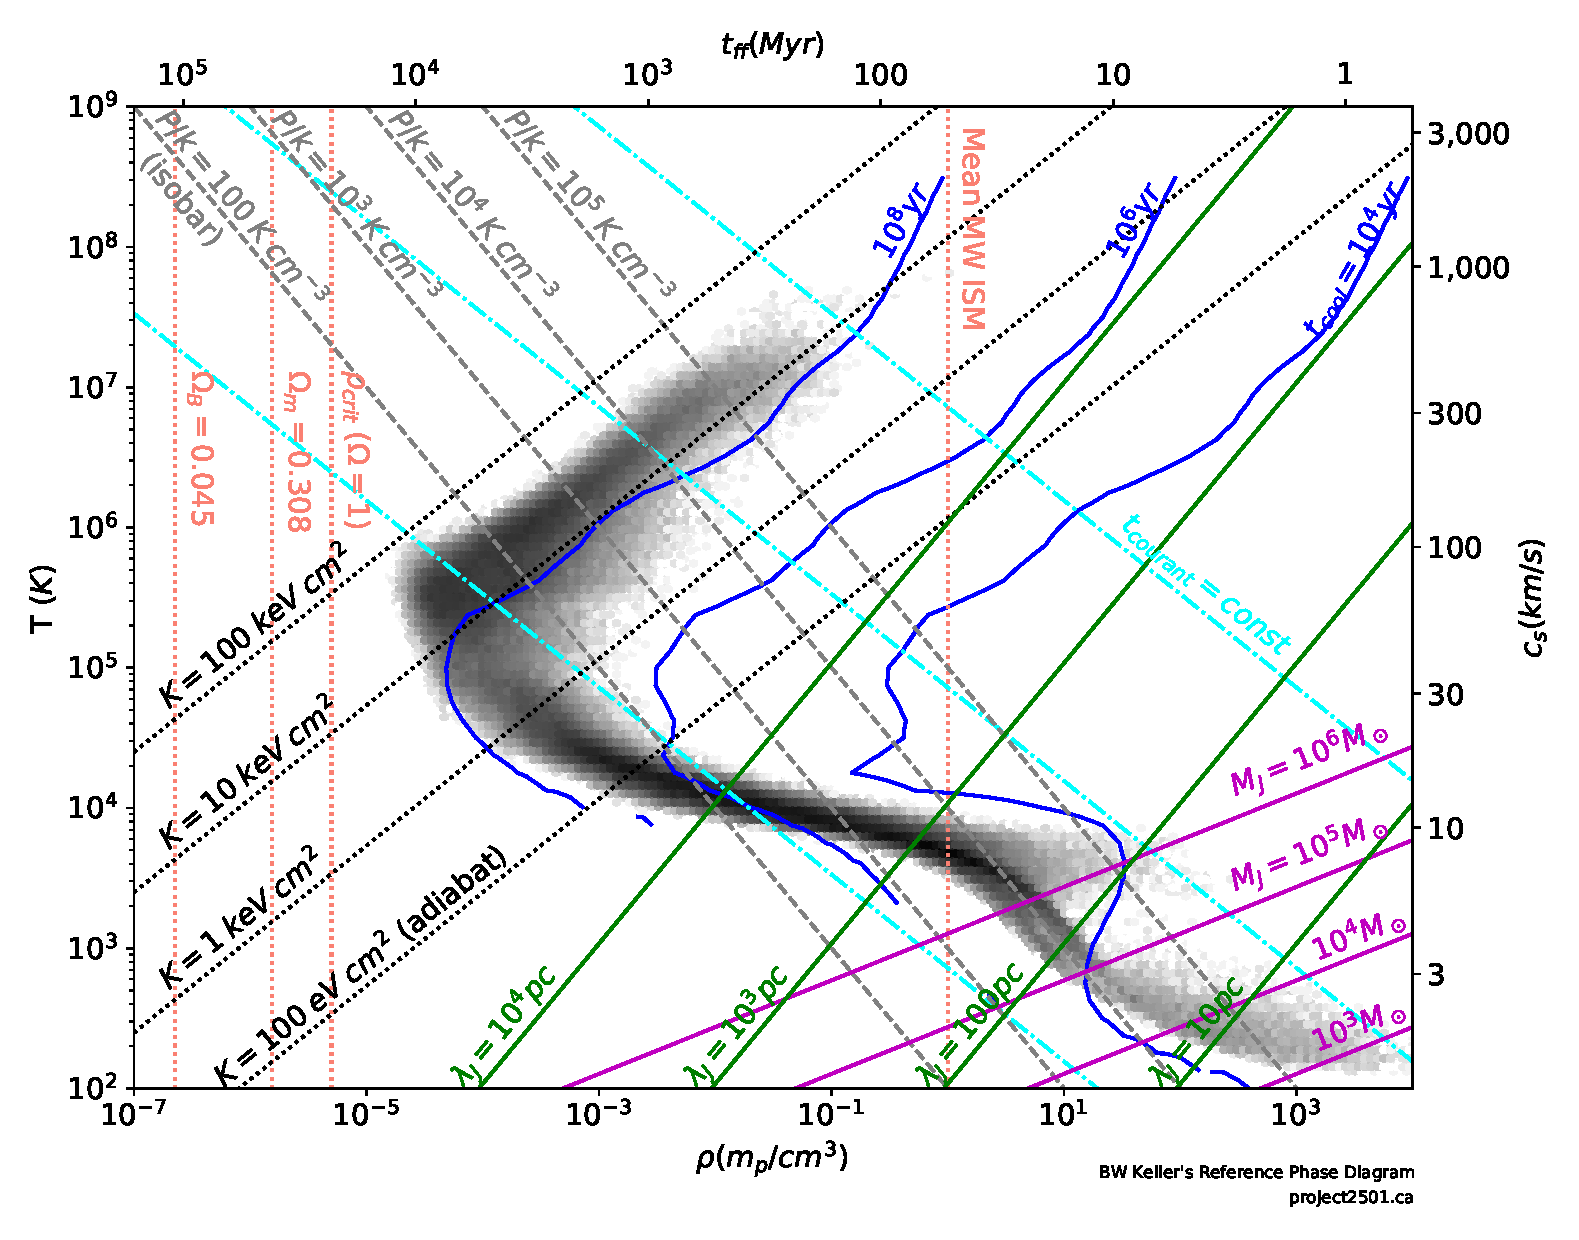
\includegraphics[width=11in]{phase_guide.eps}
\end{figure}
\end{document}
